\subsection{Social network estimation from multiple visual sources}
\label{sec:vis2net}

In the previous two sections, we presented two core problems on extracting socialized visual representations: Detection and recognition of social interaction categories, and learning new social interaction categories. In this section, we propose the paradigm by which we sense the network from visual representations. To this end, note that the most fundamental problem in social network may be probably how to represent such a network, and only with a good representation one is able to perform learning and inference in a practical manner. An undirected weighted graph $G$ of $K$ nodes, with a non-negative weight associated with each edge between a pair of nodes, has been dominantly used to represent a community of $K$ members, where the weight depicts the closeness, or ties, between the two member. Despite the effectiveness and efficiency of such a representation, we envisage and have justified in the introduction that such models can be significantly enriched by introducing visual sensors, and we argue that a more appropriate network representation should account for realistic conditions arising from not only visual but also other conventional information sources. We propose in this section a new framework by which we re-represent a visually sensed social network in a realistic world.

First, the description of a network is generally in multiple views from visual sensors and even multiple types of conventional sensors.  A view may refer to a specific type of attribute or feature or cues computed by a particular computer vision algorithm. The social relationship between two humans, for example, can be in three views: whether they participate in a social interaction as detected by Section \ref{sec:activity}, the number of their co-occurrence in pictures, and their relative gazes in images as estimated by a gaze estimator. In this case, each type of image features or attributes explicitly corresponds to a view in the network representation, and we may directly reach a three-view network representation $G\triangleq\{A^{(1)}, A^{(2)}, A^{(3)}\}$, where the matrix $A^{(i)}, i=1,2,3$ is a symmetric affinity matrix describing the closeness or ties between every pair of two members in the $i$th view. In this case, the affinity weight comes directly or via simple heuristic derivation from the visual features computation. 

However, this may not be true, when the available types of low-level visual cues are much more than the number of views of interest, and in particular, when the views of the network correspond to higher-level semantics that are not directly or explicitly related to the low-level visual cues. Consider a similar example, where we have successfully detected and tracked two faces $i$ and $j$, and through the state-of-art computer vision techniques we have computed a set of five descriptors characterizing five types of visual cues, including: 1) Relative positions of the two detections (denoted as $\vy^1$, where $\vy^1(i,j)$ denotes the relative poses between human $i$ and human $j$. The same notion applies for the remaining visual cues.); 2) mutual gazes (denoted as $\vy^2$); 3) mutual body poses (denoted as $\vy^3$); 4) their participation in social interactions (denoted as $\vy^4$); and 5) scene classification (denoted as $\vy^5$). The network we expect to estimate, on the other hand, is a three-view network, where $A^{(1)}, A^{(2)}, A^{(3)}$ all take values in $[0,1]$ indicating the probabilities of the two individuals belonging to the specific types of relationship: friend, family, and workmates. At their extreme values, $A^{(1)}(i,j)=1$ means the two people are friends and $A^{(1)}(i,j)=0$ means that they do not get along with each other well,  $A^{(2)}(i,j)=1$ means the two people definitely belong to the same family and $A^{(2)}(i,j)=0$ means otherwise, and $A^{(3)}(i,j)=1$ means the two people are workmates and $A^{(2)}(i,j)=0$ means otherwise. In this example, it is unclear how we may derive the binary socially-characteristic quantities $A$'s from the low-level clues $\vy^1$ to $\vy^5$.  Moreover, these high-level views almost always embeds community structures, meaning that the members belongs to different clusters in each view, within each of which the members share close ties with each other, and members from different clusters are different from each other. To explain this, consider a network of members who are mutually each others family members, workmates, or friends. Apparently, the clustering patterns for the families, for the career, and for friendship are all different, while each member can be fully situated in each and every of these types of communities.

Regardless of whether the views depict low-level visual ties or high-level relationship communities, we seek an unified learning-based paradigm to obtain the multi-view network representations (affinity matrices) from the multiple low-level heterogeneous visual cues. We refer to this architecture as multi-view network estimation from multiple low-level visual sources. In general, we assume that there exist $S$ types of low-level `sensors' which provide $S$ types of descriptors $\vy^s, s=1,2,\cdots,S$, where $\vy^s(i,j)$ denotes the description about the pairwise or relative visual cues between human $i$ and human $j$, and these visual cues are relevant to high-level social semantics of the network of $V$ views $A^{(v)}, v=1,2,\cdots,V$. Our architecture consists of $S\times V$ `oracles' $\Psi_{s,v}$, each of which is an estimator $\hat{A}^{(v)}$ of view $v$ from descriptor $\vy^s$, i.e., $\hat{A}^{(v)}=\Psi_{s,v}(\vy^s)$. To learn the optimal `oracles', let us assume that we have $N$ `ground-truth' graphs $G_1, G_2, \cdots, G_N$ (These ground-truths are available, for instance, through our prototype system as to be introduced in Section \ref{sec:sys}) associated with their visual cues $\vy^{s}_{n}, s=1,2,\cdots,S, n=1,2,\cdots,N$ computed from related imagery. Then, the overall learning objective can be represented as 
\begin{equation}\label{eq:sensing}
\{\Psi^{*}_{s,v}\}=\arg\min_{\{\Psi_{s,v}\}}\sum_{n=1}^{N}\mathcal{J}(\{\Psi_{s,v}\}, \{\vy^{s}_n\}, \{A^{(v)}_n\})+\sum_{n=1}^{N}\tau(\{\hat{A}^{(v)}_n\})+\gamma(\{\Psi_{s,v}\}).
 \end{equation}
 
Specifically, we use the first term $\mathcal{J}$ to enforce the estimation quality of the oracles, for example, by defining
\begin{equation}\label{eq:L2error}
\mathcal{J}(\{\Psi_{s,v}\}, \{\vy^{s}_n\}, \{A^{(v)}_n\})=\sum_{s=1}^{S}\sum_{v=1}^{V}\|\Psi_{s,v}(\vy^{s}_n)-A^{(v)}_n\|^{2},
 \end{equation}
such that the estimated network is as close as possible to the `ground-truth' in the sense of minimal $l_2$ error between the affinity matrices. One may image that a conventional regression suffices for this purpose, and powerful regression machines exist, such as support vector regression, Gaussian process regression, as well as deep learning. However, socially-compatible estimations requires more than conventional estimations, in the sense that the individual oracles must give compatible estimates across views. Two nodes inferred as family members by one oracle, for example, should receive low confidence score from the friendship oracle which claims that they are adversary to each other. We use the penalty $\gamma$ to enforce the compatibility among oracles. Finally, we have been fully aware of the community clustering effects of real-world social networks, and therefore we incorporate penalty $\tau$ as well to enforce the clustering effect within the estimated affinity matrix, so that if node $i$ and node $j$ are both inferred as family members of node $k$ we will have the same inference for the relationship between $i$ and $j$. We omit further discussion about $\gamma$ and $\tau$ due to space limitation.


%\begin{figure}[t!]
%\begin{center}
%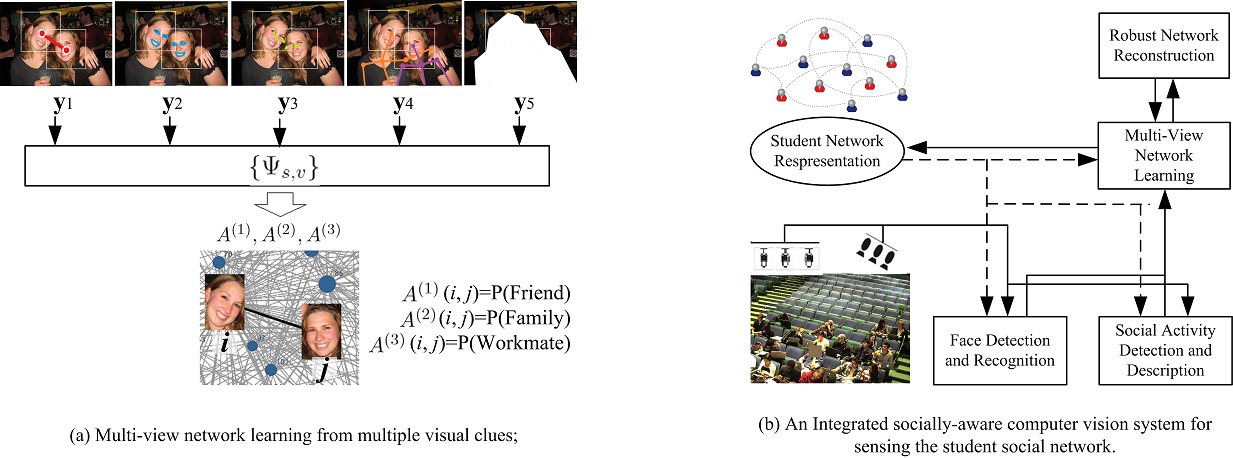
\includegraphics[width=\columnwidth]{featurelearn}
%\end{center}
%\vspace{-0.25in} \caption{\captionsize 
%Illustrations for the problem of multi-view network learning from multiple low-level visual clues and the framework of integrated socially-aware computer vision for understanding student netwrok. \label{fig:featurelearn}\afterfigspace}
%\end{figure}


We argue that cross-view compatibility and within-view clustering are essential to any socially-aware `sensors' or computational machines that aim to estimate the social attributes from low-level visual cues, or even other types of conventional clues. This socially-aware sensing architecture, dissimilar to any other regression machines which take in and output independent samples, is at the heart of our proposed social visual sensing paradigm.



%%%%%%%%%%%%%%%%%%%%%%%%%%%%%%%%%%%%%%%%%%%%%%%%%%%%%%%%%

\subsubsection{Robust Face Identity Association}
\label{sec:assoc}

To obtain the low-level visual descriptions $\vy^s$ between individual $i$ and individual $j$, we must first identify the two individuals from the detections in images or tracks in videos. While the state-of-art face recognizer has achieved compellingly outstanding performance even for the faces `in the wild', there always remain ambiguities and errors. Suppose that from an image we have detected $L$ faces or from a video we have tracked $L$ faces, and we must assign each of these $L$ targets to one of the possible $K$ identities of interest for the social network estimation approach to work. We propose to explore robust algorithms that may properly handle the non-robustness of a face recognizer and provide identity assignments that are less sensitive to the erroneous output from a face recognizer.

While we aim to develop and evaluate many possible solutions and finally determine the optimal one during the award period, a preliminary solution can be straightforward. Instead of assigning each target to a single identity from $K$ possible ones that might be incorrect, consider that the face recognizer outputs a $K$-dimensional probabilistic histogram $h_l$ for the $l$th target in the image or video, with $h_m(k)$ describing the likelihood for this target to belong to the $k$th identity. To leverage and properly aggregate these likelihood conveyed from face recognition, we may first enumerate all $\prod_{l=0}^{L-1}(K-l)$ possible assignments. We then may duplicate the original image or video into $\prod_{l=0}^{L-1}(K-l)$ copies, in each of which we may assume that the $L$ targets have a determined identity assignment $\{k_1, k_2, \cdots, k_L\}, k_l\in\{1,2, \cdots, K\}$. We allow all these $\prod_{l=0}^{L-1}(K-l)$ `hallucinated' samples to be used for computing low-level description $\vy^s$, where the $(i,j)$-pair of targets will contribute to the descriptor $\vy^s(k_i,k_j)$, with appropriate pooling strategy to effective and efficiently aggregate all contributions from the expanded set of $\prod_{l=0}^{L-1}(K-l)$ new samples.


A `maximum-pooling' approach, for example, may be employed by determining $k_l^{*}=\max_{k}h_l(k)$, the most probable identity for target $l$, and use the only maximum assignment $\{k_1^{*}, k_2^{*}, \cdots, k_L^{*}\}$ to compute the visual cues between individuals specified by $\{k_1^{*}, k_2^{*}, \cdots, k_L^{*}\}$. This strategy is essentially identical to the idea of assigning each target to a single (possibly incorrect) identity. Alternatively, we may adopt a weighted average pooling, where the hallucinated image/video with assignment $\{k_1, k_2, \cdots, k_L\}$ will contribute to the visual cues but with a confidence score, for example, of $\prod_{l=1}^{L}h_l(k_l)$.

It is critical for our overall framework to be equipped with an optimal identity association and pooling mechanism, especially when we aim to accumulate social evidence from many image/video samples. We propose to evaluate all possible solutions and report the optimal solution during the research activity.